\documentclass[article]{article}
\usepackage[utf8]{inputenc}
\usepackage[english]{babel}

\usepackage[backend=biber,
style=authoryear,
citestyle=apa]{biblatex}
\addbibresource{refs.bib}

%% Sets page size and margins
\usepackage[letterpaper,top=3cm,bottom=2cm,left=3cm,right=3cm,marginparwidth=1.75cm]{geometry}
 
%% Useful packages
\usepackage{amsmath}
\usepackage{amssymb}
\usepackage{amsfonts}
\usepackage{mathtools}
\usepackage{graphicx}
\usepackage{enumitem}
\usepackage{hyperref}
% \usepackage{pythontex}
\usepackage{lastpage}
\usepackage{fancyhdr}
\usepackage{float}
\usepackage{csquotes}
% \usepackage{fontspec}
\usepackage{indentfirst}

\pagestyle{fancy}
\graphicspath{ {images/} }
\newcommand{\true}{$T$}
\newcommand{\false}{$F$}
\newcommand{\ans}{\textbf{Answer: }}
\newcommand{\prf}{\textbf{Proof:}}
\newenvironment{question}[2][Question]{\begin{trivlist}
\item[\hskip \labelsep {\bfseries #1}\hskip \labelsep {\bfseries #2.}]}{\end{trivlist}}

\let\emptyset\varnothing

\newenvironment{myindentpar}[1]%
  {\begin{list}{}%
          {\setlength{\leftmargin}{#1}}%
          \item[]%
  }
  {\end{list}}

\allowdisplaybreaks

\title{STAT 490, Final Project Proposal} 
\lhead{STAT 490, Final Project Proposal}

\author{Elnard Utiushev, Jessica Lynn Gilbert, Elijah Higgins}
\rhead{Elnard Utiushev, Jessica Lynn Gilbert, Elijah Higgins}
\cfoot{\thepage\ of \pageref{LastPage}}

\begin{document}

\maketitle

\tableofcontents

%% Comments
% - Paper meta analysis!!!
% - Collect case reports and do lexical analysis. Word freq.
%   - ARDS
% . - ARDS outbreak 2003
%   - MRIS


\section{Introduction}
% - e-cigarettes became popular in (year) as what was thought to be a "safe" alternative to tobacco products
% - However, towards the beginning of (2019) there have been a stark increase in the number of serious injuries and deaths believed to be caused by these e-cigs
% - because it's a hot topic right now, lots of conflicting information is circulating about the dangers of e-cigs
% - our study will shed light on what's *actually* going on

E-cigarettes have become popular in recent years (Figure \ref{fig:vape_trend}) as what was thought to be a "safe" alternative to tobacco products. However, toward the beginning of 2019 there have been a sudden increase in the number of serious injuries and deaths believed to be caused by these e-cigarettes (\cite{doi:10.1056/NEJMoa1911614}).
 
The effects of vaporizer and e-cigarette use is currently a "hot topic" and a lot of conflicting information is circulating through media and research studies. As a result, many people are unsure of whether they can trust these new tobacco alternatives.
 
Our prospective cohort study will investigate the differences in effects of tobacco cigarettes, nicotine-infused e-cigarettes, nicotine-free e-cigarettes, THC-infused e-cigarettes, and no cigarette use.

\begin{figure}[H]
    \centering
    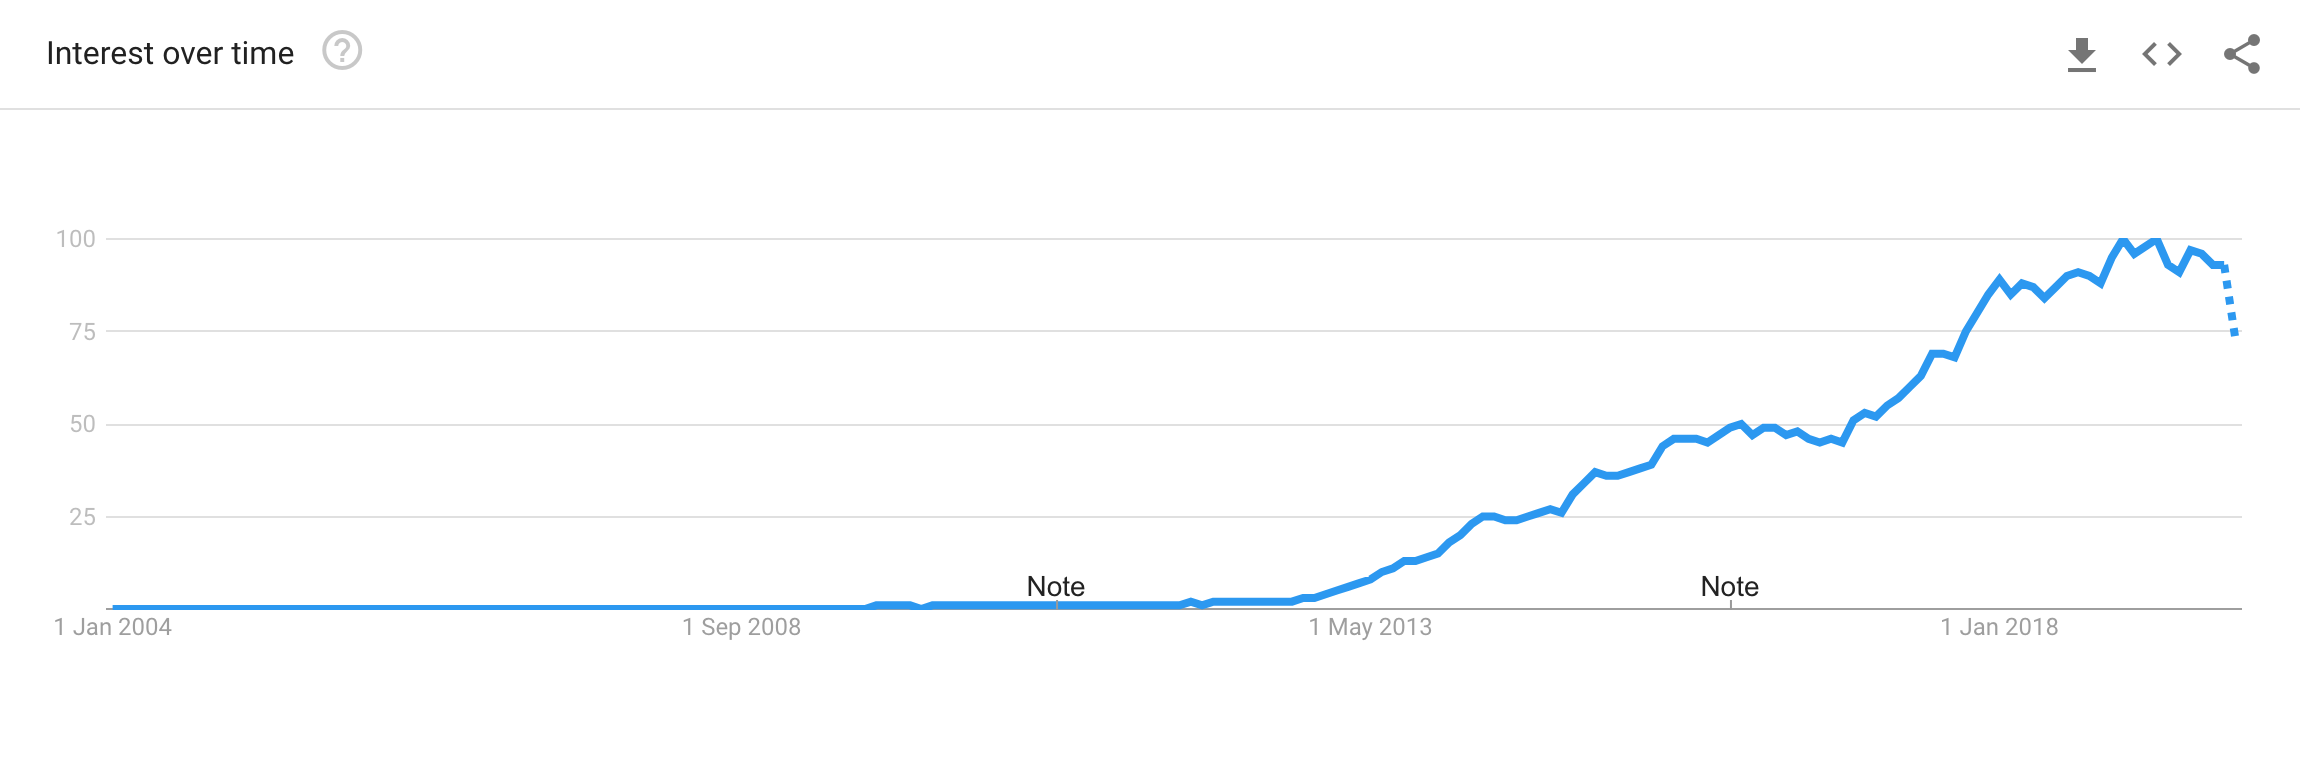
\includegraphics[width=\columnwidth]{google_trends_vape.png}
    \caption{\href{https://trends.google.com/trends/explore?date=all&geo=US&q=vape}{Google Trends Data for "vape" keyword} (\cite{google_trends})}
    \label{fig:vape_trend}
\end{figure}

\section{Literature Review}
% Paper on effects of vaping: https://onlinelibrary.wiley.com/doi/full/10.1111/add.14530
% Their design was a cohort-specific simulation model of the impact of replacing smoking with nicotine vaporizing products. Their participants included two cohorts aged 30 and 50 in 2012.
% They concluded that NVP's would have a net positive impact on population health.

In 2019, a paper was published on the effects of smoking (\cite{levy2019modeling}). Their study looks at two cohorts made up of participants aged 30 and 50 in 2012 who had known smoking patterns. Their goal was to determine what impacts replacing smoking with nicotine vaporizing products (NVP) would have. They use data on the history of smoking for each cohort to make two simulations: one which they model smoking rates for each cohorts life cycle in the absence of vaping and one model which considers the effects of vaping. Their study found that participants in the younger cohort had fewer paper premature deaths and life-years lost, in the presence of NVP's.

\medskip

A paper in 2018 investigated the potential of e-cigarettes as an alternative to tobacco cigarettes. (\cite{Levy18})
Here is their description of their methods: 

\begin{displayquote}
A Status Quo Scenario, developed to project smoking rates and health outcomes in the absence of vaping, is compared with Substitution models, whereby cigarette use is largely replaced by vaping over a 10-year period. We test an Optimistic and a Pessimistic Scenario, differing in terms of the relative harms of e-cigarettes compared with cigarettes and the impact on overall initiation, cessation and switching. Projected mortality outcomes by age and sex under the Status Quo and E-Cigarette Substitution Scenarios are compared from 2016 to 2100 to determine public health impacts.
\end{displayquote}

At the end of their study, researchers concluded that the replacement of tobacco cigarettes with e-cigarettes is projected to lower overall harm to smokers based on the results of both scenarios.

\medskip

We also found a new paper by \cite{doi:10.1056/NEJMoa1911614} that explored the recent deaths caused by pulmonary illnesses in people who vaped. They did a case study on 53 patients. All of the patients had bilateral infiltrates.

\section{Research Design and Methods}
%We will do something and then something else and a third thing and maybe a fourth maybe even a fifth thing, throw in some devils lettuce and thats a study.
We will perform a literature analysis in which we investigate the publications above and the accuracy of their methods and results.



\clearpage
% \medskip
 
\addcontentsline{toc}{section}{References}
\printbibliography

\end{document}
